\documentclass[11pt,letterpaper,twocolumn]{article}

\usepackage[utf8]{inputenc}
\usepackage{tcolorbox} 
\usepackage[spanish]{babel}
\usepackage{float}
\usepackage{xcolor}
\usepackage{verbatim}
\usepackage{mwe}
\usepackage{charter}
\usepackage{afterpage}
\usepackage{amsmath}
\usepackage{appendix}
\usepackage{ragged2e}
\usepackage{array}
\usepackage{etoolbox}
\usepackage{fancyhdr}
\usepackage{booktabs}
\usepackage{arydshln}
\usepackage[justification=justified,singlelinecheck=false,labelfont=bf,format=plain]{caption}
\usepackage[justification=justified,singlelinecheck=false,labelfont=bf,format=plain]{subcaption}
\usepackage{enumitem}
\usepackage[bottom=2.5cm,top=2.0cm,left=2.0cm,right=2.0cm]{geometry}
\usepackage{graphicx}
\usepackage{indentfirst}
\usepackage{mathtools}
\usepackage{multirow}
\usepackage{pdfpages}

\usepackage{subfiles}
\usepackage[compact]{titlesec}
\usepackage{blindtext}
\usepackage{stfloats}
\usepackage{lipsum} 


\renewcommand{\familydefault}{\rmdefault}

\newcommand\blankpage{
    \null
    \thispagestyle{empty}
    \addtocounter{page}{0}
    \newpage}

\newcolumntype{L}[1]{>{\raggedright\let\newline\\arraybackslash\hspace{0pt}}m{#1}}
\newcolumntype{C}[1]{>{\centering\let\newline\\arraybackslash\hspace{0pt}}m{#1}}
\newcolumntype{R}[1]{>{\raggedleft\let\newline\\arraybackslash\hspace{0pt}}m{#1}}

    \setlist[itemize,1]{label=$\bullet$}
    \setlist[itemize,2]{label=$\circ$}
    \setlist[itemize,3]{label=$-$}
    \setlist{nosep}

\setlength{\columnsep}{30pt}

\titlelabel{\thetitle.\quad}

\pagestyle{fancy}
\fancyhf{}
      
\fancyfoot{}
\fancyfoot[C]{\thepage} % page
\renewcommand{\headrulewidth}{0mm} % headrule width
\renewcommand{\footrulewidth}{0mm} % footrule width

\makeatletter
\patchcmd{\headrule}{\hrule}{\color{black}\hrule}{}{} % headrule
\patchcmd{\footrule}{\hrule}{\color{black}\hrule}{}{} % footrule
\makeatother

\definecolor{blueM}{cmyk}{1.0,0.49,0.0,0.47}

%%%%%%%%%%%%%%%%%%%%%%%%%%%%%%%%%%%%%%%%%%%%%%%%%%%%%%%%%%%%%%%%%%%%%%%%%%%%%%%%%%%%%%%%%%%%%%%%%%%%%%%%%%%%%%%%%%%%%%%%%%%%%%%%%%%%%%%%%%%%%%%%%%%%%%%%%%%%%%%%%%%%%%%%%%%%%%%%%%%%%%%%%%%%%%%%%%%%%%%%%%%%%%
%%%%%%%%%%%%%%%%%%%%%%%%%%%%%%%%%%%%%%%%%%%%%%%%%%%%%%%%%%%%%%%%%%%%%%%%%%%%%%%%%%%%%%%%%%%%%%%%%%%%%%%
\title{Práctica 1: Transformadores }
\author{Álvaro Martín Romero \\
Manuel Pérez Luna\\
Roberto Rodríguez Vaz}
\begin{document}
\twocolumn[\begin{@twocolumnfalse}
\maketitle
\centerline{\rule{0.95\textwidth}{0.4pt}}

\begin{center}
    
    \begin{minipage}{0.9\textwidth}
        % RESUMEN
        \noindent \textbf{Objetivo:} El objetivo de la práctica es entender el funcionamiento de los transformadores  eléctricos y estudiar como, mediante la ley de Lenz y Faraday, sirven para transformar una corriente alterna de una intensidad y tensión dada en otra corriente con diferente intensidad y tensión

        \vspace{4mm}
        % PALABRAS CLAVE
        \noindent \textbf{Palabras clave:} Transformadores, corriente alterna, intensidad y tensión
    
    \end{minipage}
    
\end{center}
\centerline{\rule{0.95\textwidth}{0.4pt}}
\vspace{15pt}
\end{@twocolumnfalse}]
%%%%%%%%%%%%%%%%%%%%%%%%%%%%%%%%%%%%%%%%%%%%%%%%%%%%%%%%%%%%
\section{Introducción}
\justify
Un transformador es un elemento eléctrico que altera, aumentando o disminuyendo  la tensión en un circuito eléctrico  de corriente alterna manteniendo la  potencia. Está  constituido por dos bobinas independientes unidas por un núcleo  de hierro  formado por la superposición  de láminas  aisladas para evitar  las corrientes de Foucault. Un esquema de un transformador es el siguiente:
\begin{figure}[H]
	\centering
	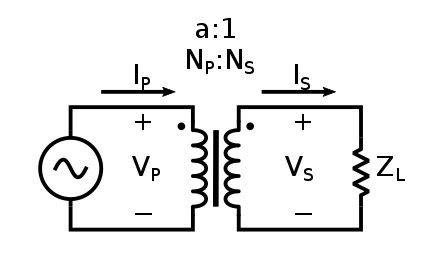
\includegraphics[width=0.4\textwidth]{transformador.png}
	\caption{Esquema de un transformador formado por dos bobinas independientes unidas entre sí}
	\label{fig:transformador-png}
\end{figure}

Al existir un elemento ferromagnético entre las dos bobinas, el flujo magnético  que atraviesan ambas bobinas es el mismo, de forma que, según la ley de Faraday:
\begin{equation}
	\varepsilon_1=-n_1 \frac{d \phi_1 }{d t}; \; \; \;  \varepsilon_2=-n_2 \frac{d \phi_2}{d t}
\end{equation}
con $\phi_1= \phi_2$ \\
\\
De esta forma, las diferencias de potencial entre  los dos arrollamientos es :
\begin{equation}
	\frac{V_1}{n_1}=\frac{V_2}{n_2}
\end{equation}
Debido a la conservación de la potencia:
\begin{equation}
	I_1n_1=I_2n_2		
\end{equation}
Estas expresiones  son las que  investigaremos de forma experimental
\section{Resultados}%
\label{sec:}
\subsection{Relaciones entre tensiones en el primario y el secundario}%
\label{sec:}
Medimos experimentalmente el valor de las tensiones de salida y entrada y representamos gráficamente $V_2$ frente a $V_1$ para hallar el valor de la pendiente para cada $n$ diferente:
\newpage
\begin{itemize}
	\item[1]: \textbf{Para n=450}
		\begin{table}[H]
			\centering
			\caption{Valores hallados experimentalmente para $n=450$ de la tensión de salida $V_2$ para cada $V_1$}
			\begin{tabular}{|c|c|}
				\hline
				\multicolumn{1}{|l|}{$V_1 \pm 0.01 V$} & \multicolumn{1}{l|}{$V_2 \pm 0.01 V$} \\ \hline
				0,38 & 0,35 \\ 
				1,07 & 1,01 \\ 
				1,45 & 1,36 \\ 
				2,08 & 1,96 \\
				3,74 & 3,56 \\
				4,56 & 4,34 \\
				5,62 & 5,35 \\ 
				6,63 & 6,45 \\
				7,75 & 7,44 \\
				8,82 & 8,47 \\
				9,68 & 9,32 \\
				10,36 & 9,96 \\ \hline
			\end{tabular}
			\label{}
		\end{table}

			Representando gráficamente:

\begin{figure}[H]
			\centering
			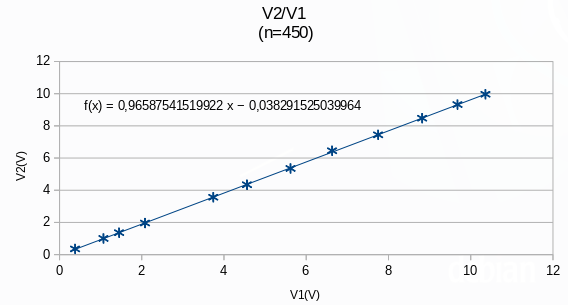
\includegraphics[width=0.5\textwidth]{v450.png}
			\caption{Representación gráfica de $V_2$ frente a $V_1$}
			\label{fig:v2v1450-png}
		\end{figure}
\end{itemize}

Haciendo la estimación lineal nos queda que la pendiente es:

\begin{equation}
	\boxed{V_2={\left( 0.97\pm 0.03 \right)\cdot V_1 - \left( 0.040 \pm 0.018 \right)} (V)  }
\end{equation}



\item[2]: \textbf{Para n=900}
		\begin{table}[H]
			\centering
			\caption{Valores hallados experimentalmente para $n=900$ de la tensión de salida $V_2$ para cada $V_1$}
			\begin{tabular}{|c|c|}
				\hline
				\multicolumn{1}{|l|}{$V_1 \pm 0.01 V$} & \multicolumn{1}{l|}{$V_2 \pm 0.01 V$} \\ \hline
				0,38 & 0,69 \\ 
				1,37 & 2,59 \\ 
				2,68 & 5,09 \\
				3,77 & 7,19 \\
				4,37 & 8,31 \\
				5,32 & 10,2 \\
				5,71 & 10,96 \\
				6,64 & 12,7 \\
				7,64 & 14,66 \\ 
				8,29 & 15,9 \\ 
				9,68 & 18,6 \\ 
				10,12 & 19,5 \\ \hline
			\end{tabular}
			\label{}
		\end{table}

			La representación gráfica de $V_2$ frente a $V_1$ queda tal que:

		\begin{figure}[H]
			\centering
			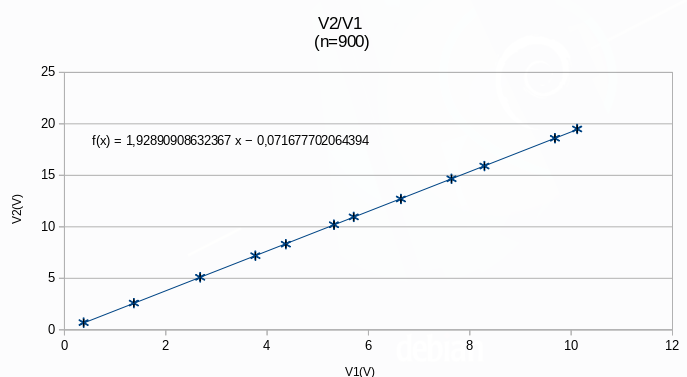
\includegraphics[width=0.6\textwidth]{v900.png}
			\caption{Representación gráfica de $V_2$ frente a $V_1$ para $n=900$}
			\label{fig:v900-png}
		\end{figure}

El valor de la recta de regresión al hacer la regresión lineal es:
\begin{equation}
\boxed{V_2={\left( 1.928 \pm 0.003 \right) \cdot V_1 -\left( 0.072 \pm 0.018 \right)} \left( V \right) }
\end{equation}
\newpage

\item[3]: \textbf{Para n=1800}
		\begin{table}[H]
			\centering
			\caption{Valores hallados experimentalmente para $n=1800$ de la tensión de salida $V_2$ para cada $V_1$}
			\begin{tabular}{|c|c|}
				\hline
				\multicolumn{1}{|l|}{$V_1 \pm 0.01 V$} & \multicolumn{1}{l|}{$V_2 \pm 0.01 V$} \\ \hline
				0,38 & 1,42 \\ 
				1,27 & 4,79 \\
				2,22 & 8,48 \\
				3,35 & 12,72 \\
				4,37 & 16,65 \\
				5,35 & 20,30 \\ 
				6,02 & 22,90 \\ 
				6,83 & 26.00 \\ 
				7,23 & 27,50 \\
				8,17 & 31,10 \\
				9,68 & 36,90 \\
				10,59 & 40,40 \\ \hline
			\end{tabular}
			\label{}
		\end{table}
		Representando gráficamente:
		\begin{figure}[H]
			\centering
			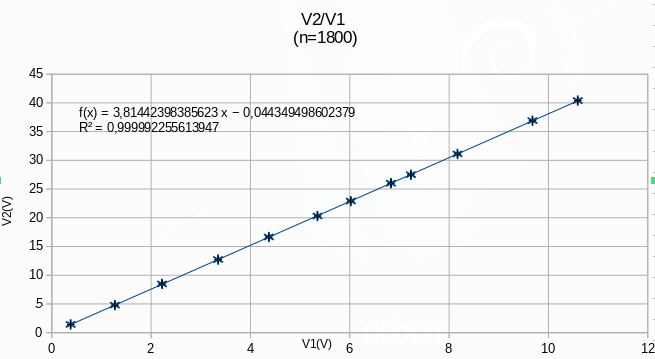
\includegraphics[width=0.5\textwidth]{v1800.png}
			\caption{Representación gráfica de $V_2$ frente a $V_1$ para $n=1800$}
			\label{fig:1800-png}
		\end{figure}

		La recta de regresión lineal es tal que :
		\begin{equation}
			\boxed{V_2={\left( 3.814 \pm 0.004 \right) \cdot V_1 -\left( 0.044\pm 0.022 \right) } \left( V \right) }
		\end{equation}

		\subsubsection{Representación de puntos comunes de $V_1$}

		A continuación representamos los datos de puntos comunes de voltaje $V_1$ entre las 3 medidas para cada $n_2$ :	\\
\\
La recta de regresión teórica es:
\begin{equation}
	V_2=(\frac{V_1}{n_1})\cdot n_2	
\end{equation}
Llamaremos $m_t=\frac{V_1}{n_1}$
		\begin{table}[H]
			\caption{Medidas de puntos comunes de $V_1$ para cada $n_2$ diferente}
			\centering
			\begin{tabular}{|c|c|c|c|}
				\hline
				\multicolumn{1}{|c|}{} & $n_2=450$ & $n_2=900$ & $n_2=1800$ \\ \hline
				$V1\pm 0.01 V$ & $V_2 \pm 0.01$ V & $V_2  \pm 0.01 V$  & $V_2 \pm 0.01 V$ \\ \hline
				0,38 & 0,35 & 0,69 & 1,42 \\ 
				6,63 & 6,45 & 12,7 & 26 \\ 
				9,68 & 9,32 & 18,6 & 36,9 \\ \hline
			\end{tabular}
			\label{}
		\end{table}
		Si representamos a continuación gráficamente $V_2$ frente a $n_2$ nos queda:
		\begin{figure}[H]
			\centering
			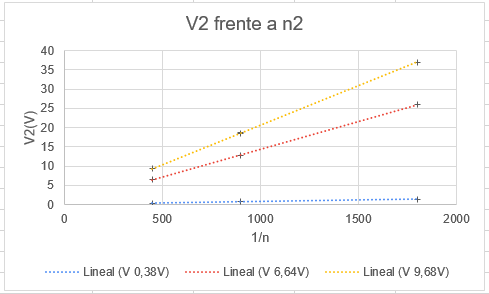
\includegraphics[width=0.5\textwidth]{vcomun.PNG}
			\caption{Representación de los puntos comunes. En línea amarilla $V_2=9.68 V$, en azul $V_2=0.38V$ y la roja $V_2=6.64V$}
			\label{fig:vcomun-png}
		\end{figure}
		La recta de regresión lineal de cada conjunto de puntos es :
		\begin{tcolorbox}[colback=yellow!5!white,colframe=yellow!75!black,fonttitle=\bfseries,title= \[
		V_1: 9.68 V
		.\] ]
		\[
			V_2=\left( 0.02042 \pm 0.00008 \right) \cdot n_2+\left( 0.17 \pm 0.09 \right) V
		.\] 	 
	\end{tcolorbox}

		El valor teórico para la pendiente es $m=\frac{V_1}{n_1}$. Sustituyendo $V_1$ y $n_1$ y haciendo error por dispersión de Gauss nos queda que el valor de la pendiente teórico es :
		\[
			m_{t}= 2.1511 \cdot 10^{-2} \pm 2.3 \cdot 10^{-5}
		.\] 
		\begin{tcolorbox}[colback=red!5!white,colframe=red!75!black,fonttitle=\bfseries,title=\[
		V_1 :6.64V 
		.\] ]
		\[
			V_2=\left(0.01452 \pm 0.00022 \right) n_2-  \left( 0.2 \pm 0.3 \right) V
		.\]  
		\end{tcolorbox}
		El valor teórico de la pendiente es:
		\[
			m_t=1.5178 \cdot 10^{-2} \pm 2.3 \cdot 10^{-5}
		.\] 

	\begin{tcolorbox}[colback=blue!5!white,colframe=blue!75!black,fonttitle=\bfseries,title= \[
	V_1: 0.38 V
	.\] ]
		\[
			V_2=\left( 7.95 \cdot 10^{-4} \pm 1.3 \cdot 10^{-5} \right) n_2 - \ldots 
		.\] 	 
		\[	
		\ldots-\left( 0.015 \pm 0.017 \right) V
		.\] 
\end{tcolorbox}
El valor teórico de la pendiente es:
\[
	m_t=8.44 \cdot 10^{-4} \pm 2.3 \cdot 10^{-5}
.\]
		\subsection{Relaciones entre intensidades entre el primario y el secundario}

		\begin{itemize}
			\item[1]: \textbf{Para n= 450} 
				A continuación expresamos los datos medidos directamente del laboratorio para $I_1$ y $I_2$ :
				\begin{table}[H]
					\centering
					\caption{Valores medidos directamente del laboratorio para $n_2=450$}
					\begin{tabular}{|c|c|}
						\hline
						$\left( I_1\pm_0.01 A \right) $ & $\left( I_2 \pm 0.01 A \right) $ \\ \hline
						0,14 & 0,13 \\
						0,25 & 0,24 \\
						0,33 & 0,32 \\
						0,45 & 0,45 \\
						0,6 & 0,59 \\ 
						0,78 & 0,76 \\
						0,85 & 0,84 \\ 
						0,97 & 0,95 \\ 
						1,1 & 1,09 \\ 
						1,2 & 1,18 \\ 
						1,28 & 1,26 \\
						1,64 & 1,62 \\ \hline
					\end{tabular}
					\label{}
				\end{table}
		 Representamos gráficamente $I_2$ frente a $I_1$ :
		 \vfill  \hfill
		 \begin{figure}[H]
		 	\centering
		 	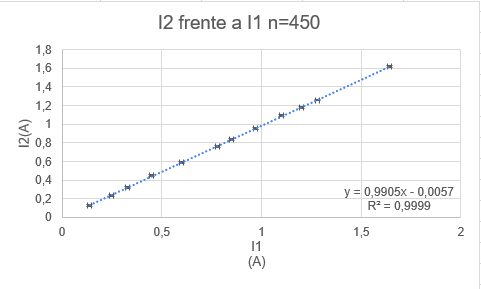
\includegraphics[width=0.5\textwidth]{In=4502.png}
			\caption{Representación gráfica de $I_2$ frente a $I_1$ para $n_2=450$}
		 	\label{fig:In-4502-png}
		 \end{figure}
		La recta de regresión lineal es:
		\begin{equation}
			\boxed{I_2={\left( 0.990 \pm 0.004 \right) \cdot I_1 - (0.006 \pm 0.004) } \left( A \right)  }
		\end{equation}
		
			\item[2]: \textbf{Para $n_2=900$} 
				A continuación expresamos los datos medidos directamente del laboratorio para $I_1$ y $I_2$ :
				\begin{table}[H]
					\centering
					\caption{Valores medidos directamente del laboratorio para $n_2=900$}
					\begin{tabular}{|c|c|}
						\hline
						$\left( I_1\pm_0.01 A \right) $ & $\left( I_2 \pm 0.01 A \right) $ \\ \hline
						0,14 & 0,05 \\ 
						0,23 & 0,1 \\ 
						0,36 & 0,17 \\
						0,45 & 0,21 \\
						0,54 & 0,26 \\
						0,78 & 0,38 \\
						0,87 & 0,42 \\
						0,97 & 0,47 \\
						1,1 & 0,54 \\ 
						1,24 & 0,61 \\
						1,34 & 0,66 \\
						1,66 & 0,82 \\ \hline
					\end{tabular}
					\label{}
				\end{table}
		Representando gráficamente:
		\begin{figure}[H]
			\centering
			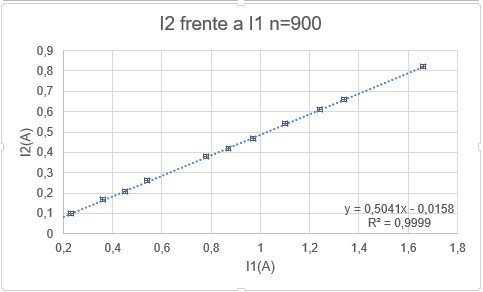
\includegraphics[width=0.5\textwidth]{In=900.png}
			\caption{Representación gráfica de $I_2$ frente a $I_1$ para $n_2=900$}
			\label{fig:In-900-png}
		\end{figure}
	La recta de regresión lineal es tal que:
	\begin{equation}
	\boxed{I_2={\left( 0.5041 \pm 0.019 \right) \cdot I_2 - \left( 0.0158 \pm 0.0017 \right)}V }
	\end{equation}


			\item[3]: \textbf{Para $n_2=1800$} \\ 

				A continuación expresamos los datos medidos directamente del laboratorio para $I_1$ y $I_2$ :
				\begin{table}[H]
					\centering
					\caption{Valores medidos directamente del laboratorio para $n_2=1800$}
					\begin{tabular}{|c|c|}
						\hline
						$\left( I_1\pm_0.01 A \right) $ & $\left( I_2 \pm 0.01 A \right) $ \\ \hline
						0,14 & 0,02 \\ 
						0,24 & 0,04 \\
						0,37 & 0,07 \\
						0,50 & 0,11 \\ 
						0,64 & 0,14 \\
						0,78 & 0,18 \\
						0,89 & 0,21 \\
						0,98 & 0,23 \\
						1,10 & 0,26 \\
						1,18 & 0,28 \\
						1,31 & 0,38 \\
						1,65 & 0,40 \\ \hline
					\end{tabular}
					\label{}
				\end{table}
				
				Representamos gráficamente:
				\begin{figure}[H]
					\centering
					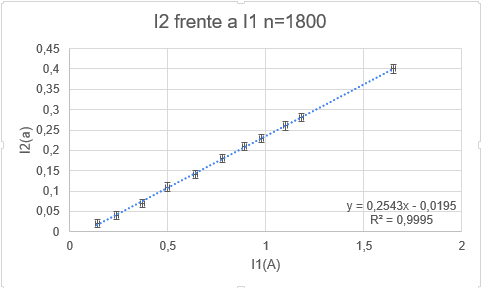
\includegraphics[width=0.5\textwidth]{In=1800.png}
					\caption{Representación gráfica de $I_2$ frente a $I_1 $ para $n=1800$}
					\label{fig:In-1800-png}
				\end{figure}
				La recta de regresión es :
				\begin{equation}
					\boxed{I_2={\left( 0.268 \pm 0.013 \right) \cdot I_1 -\left( 0.026 \pm 0.012 \right) A}}
				\end{equation}
			\end{itemize}		
			\subsection{Representación de puntos comunes de $I_1$}%
			\label{sec}
			
			Representamos los datos de los puntos comunes de intensidad $I_1$ entre las 3 medidas para cada $n_2$ :\\
\\
La recta de regresión es :
\begin{equation}
	I_2=(n_1\cdot I_1) \cdot \frac{1}{n_2}
\end{equation}
	La pendiente es: $m_t=n_1\cdot I_1$
	
\begin{table}[htbp]
				\caption{Medidas de puntos comunes de $I_1$ para cada $n_2$}
				\begin{tabular}{|c|c|c|c|}
					\hline
					 & $n_2=450$ & $n_2=900$ & $n_2=1800$ \\ \hline
					$I_1 \pm 0.01 A$ & $I_2=0.01 A$ & $I_2=0.01 A$& $ I_2=0.01 A$\\ \hline
					0,14 & 0,13 & 0,05 & 0,02 \\ 
					0,97 & 0,95 & 0,47 & 0,23 \\
					1,1 & 1,09 & 0,54 & 0,26 \\ \hline
				\end{tabular}
				\label{}
			\end{table}
			

			Si representamos a continuación gráficamente $I_2$ fernte a $\frac{1}{n_2}$
			\begin{figure}[H]
				\centering
				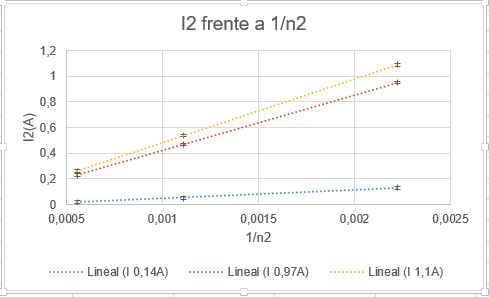
\includegraphics[width=0.5\textwidth]{icomun(1).PNG}
				\caption{Representación gráfica de puntos comunes.}
				\label{fig:icomun-1-PNG}
			\end{figure}

		La recta de regresión lineal de cada conjunto de puntos es :
		\begin{tcolorbox}[colback=yellow!5!white,colframe=yellow!75!black,fonttitle=\bfseries,title= \[
		I_1: 1.1A
		.\] ]
		\[
			I_2=\left( 498 \pm 3  \right) \cdot \frac{1}{n_2} - \left( 0.015 \pm 0.004 \right) A
		.\] 	 
	\end{tcolorbox}

		El valor teórico para la pendiente es $m=\frac{V_1}{n_1}$. Sustituyendo $V_1$ y $n_1$ y haciendo error por dispersión de Gauss nos queda que el valor de la pendiente teórico es :
		\[
			m_{t}= (495 \pm 5 ) A
		.\] 
		\begin{tcolorbox}[colback=red!5!white,colframe=red!75!black,fonttitle=\bfseries,title=\[
		I_1 :0.97A 
		.\] ]
		\[
			I_2=\left(  432,0002\pm 1\cdot 10^{-4} \right) \frac{1}{n_2} - \ldots
		\]
		\[
			\ldots-  \left( 0.0100002 \pm 1.4\cdot 10^{-7} \right) A
		.\]  
		\end{tcolorbox}
		El valor teórico de la pendiente es:
		\[
			m_t=(437 \pm 5 )A
		.\] 

	\begin{tcolorbox}[colback=blue!5!white,colframe=blue!75!black,fonttitle=\bfseries,title= \[
	I_1: 0.14 A
	.\] ]
		\[
			I_2=\left( 67 \pm 5  \right) \frac{1}{n_2} - \ldots 
		.\] 	 
		\[	
		\ldots-\left( 0.020 \pm 0.007 \right) A
		.\] 
\end{tcolorbox}
El valor teórico de la pendiente es:
\[
	m_t=(63 \pm 5) A
.\]
\section{Error de Gauss}%
\label{sec:Error de Gauss}
Exponemos a continuación los cálculos de errores utilizados:
\begin{equation}
	\Delta \left( \frac{V_1}{n_1} \right) =\sqrt{\left( \frac{1}{ n_1} \right) ^2\cdot (\Delta V_1)^2} 
\end{equation}
Para la medida de la pendiente teórica de la intensidad:
\begin{equation}
	\Delta \left( n_1\cdot I_1 \right) =\sqrt{ n_1^2\cdot \left(\Delta I_1 \right)^2} 
\end{equation}
\section{Conclusión}%
\label{sec}
\subsection{Relaciones entre tensiones en el primario y el secundario}
Sabemos que los voltajes de entrada y de salida de un transformador están relacionados por la siguiente ecuación: $V_2=\frac{n_2}{n_1}\cdot V_1$. Esto significa que la pendiente de los distintos transformadores debe ser igual a la fracción entre el segundo arrollamiento y el primero.\\
\\
Vamos a comparar los resultados esperados con los reales:
Vemos por tanto que los resultados obtenidos son extremadamente acertados con un error relativo mínimo, aunque esperable, debido a que la ecuación mencionada corresponde para el caso de un sistema ideal, por tanto, es lógico que exista una pequeña variación (por la baja) en el valor esperado debido a las pérdidas que existen en el sistema.\\
\\
Por otro lado, se nos pide que representemos ( para valores comunes de $V_1$)$V_2$ frente  $n_2$, siguiendo la ecuación $\frac{V_2}{n_2}=\frac{V_1}{n_1}$  debiendo ser la pendiente de esta directamente proporcional al valor de $V_1$.\\  
\\
Nuevamente los resultados obtenidos son muy cercanos a los reales, donde se sigue viendo con evidencia que existe una pequeña diferencia de datos debido a que no nos encontramos en un sistema ideal, es cierto que el último dato parece disonar levemente frente a los demás este error podemos achacar a fallos humanos en la realización de la práctica o durante la toma de datos. 
\subsection{Relaciones entre corrientes en el primario y el secundario}
La relación correspondiente en entre corrientes en el transformador primario y el secundario viene dado por : $I_2=\frac{n_1}{n_2}I_1$ . En este caso, al contrario que para el voltaje, la pendiente corresponde al inverso de la fracción entre el segundo arrollamiento y el primero.\\
%\\
En este caso que los resultados obtenidos siguen teniendo un error relativo muy pequeño $<5\%$, pero sin embargo la pequeña diferencia con el valor teórico en los últimos transformadores es mayor que la teórica, lo cual es físicamente imposible, por consiguiente en este caso esta diferencia ha podido darse por fallos humanos en la realización de la práctica o durante la toma de datos. \\
\\
 Por último, se nos pide que representemos ( para valores comunes de $I_1$) $I_2$ frente $\frac{1}{n_2}$ , siguiendo la ecuación $I_2n_2=n_1I_1$ debiendo ser la pendiente de esta directamente proporcional al valor de $I_1$.\\
 %\\
 Viendo estos resultados y sus errores relativos correspondientes (que no superan el $5\%$) podemos asegurar que se ha realizado un correcto procedimiento y una excelente toma de datos.\\
 \\
 Finalizando, puesto que nuestro objetivo es comprobar el funcionamiento de los transformadores y verificar las ecuaciones que lo rigen, podemos concluir que hemos obtenido unos resultados muy fieles a los reales con la diferencia esperada debido a que nuestros sistemas no son ideales, manteniéndose las relaciones entre voltajes e intensidades al pasar por el transformador esperadas. 
\end{document}

